\documentclass[conference,letterpaper]{IEEEtran}
\usepackage{fontspec}
\IfFontExistsTF{Times New Roman}{\setmainfont{Times New Roman}}{\setmainfont{TeX Gyre Termes}}
\IfFontExistsTF{Arial}{\setsansfont{Arial}}{\setsansfont{TeX Gyre Heros}}
\IfFontExistsTF{Consolas}{\setmonofont{Consolas}}{\setmonofont{Latin Modern Mono}}
\usepackage{amsmath,amssymb,graphicx,booktabs,array,cite}
\usepackage[hidelinks]{hyperref}
\usepackage{xurl}
\urlstyle{same}
\graphicspath{{figures/}}
\setcounter{dbltopnumber}{1}
\hyphenpenalty=10000
\exhyphenpenalty=10000
\emergencystretch=1em
\newcommand{\OriginalClean}{98.8}
\newcommand{\OriginalBlur}{90.8}
\newcommand{\OriginalColour}{92.7}
\newcommand{\OriginalContext}{73.6}
\newcommand{\AugClean}{98.6}
\newcommand{\AugBlur}{88.8}
\newcommand{\AugColour}{91.8}
\newcommand{\AugContext}{73.4}
\newcommand{\AmerClean}{98.0}
\newcommand{\AmerBlur}{89.7}
\newcommand{\AmerColour}{86.8}
\newcommand{\AmerContext}{74.2}
\newcommand{\UnmatchedClean}{97.7}
\newcommand{\UnmatchedBlur}{93.2}
\newcommand{\UnmatchedColour}{89.7}
\newcommand{\UnmatchedContext}{75.0}
\newcommand{\AmerTN}{94}
\newcommand{\AmerFP}{2}
\newcommand{\AmerFN}{7}
\newcommand{\AmerTP}{540}
\newcommand{\AmerSensitivity}{98.7}
\newcommand{\AmerSpecificity}{97.9}
\newcommand{\AmerFone}{0.977}
\newcommand{\AmerChanged}{25.8}
\newcommand{\OriginalChanged}{26.4}

\newcommand{\AccuracyRows}{%
Original & 98.8 & 90.8 & 92.7 & 73.6 \\ \hline
Matched augmentation & 98.6 & 88.8 & 91.8 & 73.4 \\ \hline
Full context augmentation & 98.1 & 93.3 & 92.2 & 78.2 \\ \hline
AMER & 98.0 & 89.7 & 86.8 & 74.2 \\ \hline
Unmatched AMER & 97.7 & 93.2 & 89.7 & 75.0 \\ \hline%
}
\newcommand{\CleanRows}{%
Original & 0.986 & 0.983 & 0.048 & 99.5 & 99.0 \\ \hline
Matched augmentation & 0.984 & 0.981 & 0.054 & 99.1 & 99.0 \\ \hline
Full context augmentation & 0.979 & 0.975 & 0.072 & 98.9 & 97.9 \\ \hline
AMER & 0.977 & 0.973 & 0.065 & 98.7 & 97.9 \\ \hline
Unmatched AMER & 0.974 & 0.968 & 0.092 & 98.9 & 96.9 \\ \hline%
}
\newcommand{\DifferenceRows}{%
Original & -0.8 [-1.9, +0.2] & -0.6 [-1.4, +0.0] \\ \hline
Blur & -1.1 [-2.8, +0.5] & +0.9 [-0.3, +2.2] \\ \hline
Global colour & -5.9 [-8.1, -3.7] & -5.0 [-6.8, -3.4] \\ \hline
Context colour & +0.6 [-1.7, +2.9] & +0.8 [-1.6, +3.3] \\ \hline%
}
\newcommand{\SelectionRows}{%
Original & 0.01 & 0 & 0.989 \\ \hline
Matched augmentation & 0.01 & 0 & 0.976 \\ \hline
Full context augmentation & 0.01 & 0 & 0.978 \\ \hline
AMER & 0.0001 & 0.1 & 0.983 \\ \hline
Unmatched AMER & 0.01 & 0.1 & 0.980 \\ \hline%
}

\makeatletter
\newcommand{\linebreakand}{\end{@IEEEauthorhalign}\hfill\mbox{}\par\mbox{}\hfill\begin{@IEEEauthorhalign}}
\makeatother
\newcommand{\affiliation}{\IEEEauthorblockA{Department of Electrical and Information Engineering\\University of Ruhuna\\Galle, Sri Lanka}}
\begin{document}
\title{Blood Cell Detection and Leukemia Screening\\with Area Matched Evidence Regularization}
\author{\IEEEauthorblockN{C. Y. Samarasinghe}\affiliation
\and\IEEEauthorblockN{H. M. S. Muthukumari}\affiliation
\linebreakand
\IEEEauthorblockN{N. A. N. N. N. Arachchi}\affiliation
\and\IEEEauthorblockN{A. W. M. L. M. Bandara}\affiliation}
\maketitle

\begin{abstract}
Automated blood image analysis must distinguish cell localization from disease screening and examine which image regions support its predictions. We propose area matched evidence regularization for acute lymphoblastic leukemia (ALL) screening within a blood cell analysis system. During training, a ranking loss compares category support after erasing an automatic stain proposal with support after erasing equally many context pixels. The classifier uses image labels and requires one feature extraction pass at inference. On 643 previously evaluated images, it achieves \AmerClean\% accuracy across four categories, against \OriginalClean\% for training on original images. The separate cell detector achieves mean average precision 0.910 at an overlap threshold of 0.50. Controlled comparisons show that the ranking loss does not improve clean accuracy and reduces robustness to global colour changes. The contribution is a training formulation for ALL and an empirical assessment of its evidence assumption; independent patient evaluation remains necessary.
\end{abstract}
\begin{IEEEkeywords}
blood cell detection, acute lymphoblastic leukemia, evidence guided learning, image classification, source grouping
\end{IEEEkeywords}

\section{Introduction}
Microscopic blood images support the localization of red blood cells (RBCs), white blood cells (WBCs) and platelets, as well as analysis of abnormal cell patterns. Cell detection, cell subtype classification and disease screening are distinct tasks with different annotation requirements \cite{acevedo,matek,ghader}. A combined analysis system must therefore associate each output with the labels available for that task.

This study addresses blood cell detection and acute lymphoblastic leukemia screening. The Blood Cell Count and Detection (BCCD) collection supplies detection boxes, Blood Cell Images supplies normal WBC categories, and the ALL collection supplies benign and malignant labels for complete images \cite{bccd,mooney,all_data}. The latter images contain multiple cells. A field label cannot establish which detected cell is malignant. We therefore use separate detection and screening branches, reporting cell counts alongside an ALL assessment of the image.

High image accuracy alone does not establish dependable biological evidence. Related source images can inflate performance across data partitions, and acquisition or background cues can provide shortcuts \cite{kapoor,leakage_questions,geirhos}. Simply removing the background can also discard useful information \cite{viewstudy,biomarker}. This motivates a narrower question: can training encourage greater dependence on stained regions than on an equally large region of surrounding context, without requiring expert region annotations?

We contribute area matched evidence regularization for ALL screening. The formulation combines automatic stain proposals, context controls of equal area and a supervised class margin ranking loss. It operates on image labels without expert region annotations and adds no extra feature extraction pass at inference. Five controlled training variants separate augmentation, ranking and area effects, while grouped source auditing and fixed perturbations support a reproducible comparison. Together, the formulation and evaluation test whether this evidence preference improves screening within a system that also detects and counts blood cells.

\section{Related Work}
Convolutional neural networks (CNNs) have been used for blood cell recognition and ALL image classification \cite{matek,ghader}. Residual networks illustrate the benefits of learned visual representations, while You Only Look Once (YOLO) models provide compact object detection and classification implementations \cite{resnet,yolo,ultralytics}. The present work retains a YOLOv8 nano detector and uses the classification variant as a frozen feature extractor.

Evidence guided learning provides the methodological background. Ross \emph{et al.} constrain explanations through input gradients, while Chang \emph{et al.} generate object and background interventions to reduce spurious associations \cite{ross,chang}. Askari Farsangi \emph{et al.} describe an ALL pipeline sensitive to biomarkers and a learning approach that combines several images \cite{biomarker}. More recently, Evidence-RL compares evidence removal with matched nonevidence regions during reinforcement learning of models that combine vision and language \cite{evidencerl}.

Our adaptation uses a direct margin loss for four categories with stain proposals independent of the class label in multicell ALL fields. The question is whether this supervised formulation adds value beyond context augmentation alone. Table~\ref{tab:related} identifies the closest precedents and the extension evaluated here. The methodological contribution is specific to this formulation and controlled experiment; evidence guided learning and comparison of matched regions are established principles.

\begin{table}[!t]
\caption{Closest Work and the Specific Extension Tested}
\label{tab:related}
\centering\footnotesize
\begin{tabular}{@{}p{.28\columnwidth}p{.67\columnwidth}@{}}
\toprule
Work & Relationship to this study\\
\midrule
Ross \emph{et al.} \cite{ross} & Explanation constraints motivate evidence training; our penalty compares image erasures.\\
Chang \emph{et al.} \cite{chang} & Context augmentation is an explicit control; ranking must add value beyond it.\\
Askari Farsangi \emph{et al.} \cite{biomarker} & ALL screening guided by cell regions precedes this work; image labels here support field classification.\\
Huang \emph{et al.} \cite{evidencerl} & Matched evidence comparison precedes this work; we test a supervised ALL margin formulation.\\
Abdallat \emph{et al.} \cite{viewstudy} & Original and segmented ALL views motivate testing information loss instead of assuming benefit.\\
\bottomrule
\end{tabular}
\end{table}

\begin{figure*}[t]
\centering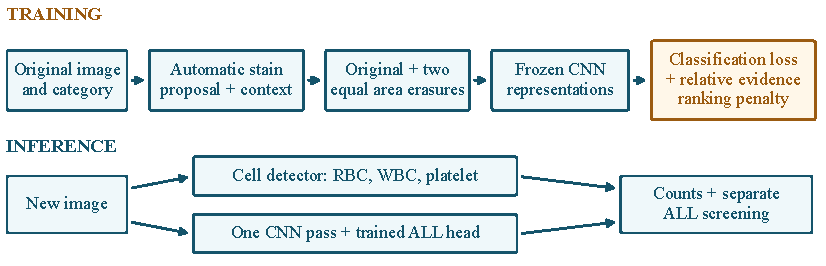
\includegraphics[width=.98\textwidth]{architecture.pdf}
\caption{Training and inference have different roles. Region interventions shape the ALL classifier during fitting. At inference, the original image supports cell detection and a separate ALL assessment. Detector boxes do not provide leukemia labels.}
\label{fig:architecture}
\end{figure*}

\section{Datasets and Source Audit}
\subsection{Cell sources and leakage correction}
BCCD contains 364 fields: 205 training, 87 validation and 72 test images. The test set contains 805 RBCs, 71 WBCs and 69 platelets. The legacy WBC split grouped augmented filenames by a random suffix rather than the original image index. Keras source code documents this naming pattern \cite{keras}. Recovering the source index showed that all 2,476 legacy validation images had augmentation relatives in training, even though their file hashes differed.

We rebuilt WBC classification from 339 original fields with one annotated WBC and one supported subtype. The partitions contain 191 training, 85 nominal validation and 63 test sources. Perceptual screening and affine registration using scale invariant feature transform (SIFT) descriptors found a related training and validation field \cite{lowe}. Excluding that validation image leaves 84 eligible fields. The new WBC classifiers use the fixed final training epoch, not a checkpoint selected using the nominal validation scores. The inherited detector's historical checkpoint selection did include this related validation scene; this limitation is retained.

\subsection{ALL images and source grouping}
The local ALL collection contains 3,256 original images at $224\times224$ pixels. The categories are Benign, Early, Pre and Pro; the malignant categories denote early pre-B, pre-B and pro-B ALL, not increasing severity \cite{ghader,all_data}. Deduplication of identical decoded pixels removes 40 copies, leaving 3,216 images.

To group observable image relatives, we compute perceptual hashes of 64 bits under eight rotations and reflections. Distances of four bits or less are grouped conservatively. Distances from five to ten additionally require affine SIFT registration, at least 12 inliers, an inlier fraction of 0.60 and image coverage of 10\%. The descriptor ratio is 0.75 and registration tolerance is three pixels. These fixed screening settings identify candidate source relationships; they do not establish patient identity. Seventy accepted links produce 3,147 groups, with no conflicting category labels. Five stratified group folds with seed 2026 assign one fold to testing, one to validation and three to training.

\begin{table}[!t]
\caption{ALL Images After Deduplication and Grouping}
\label{tab:data}
\centering\footnotesize
\begin{tabular}{@{}lrrr@{}}
\toprule Category & Training & Validation & Test\\\midrule
Benign & 305 & 103 & 96\\
Early & 587 & 200 & 198\\
Pre & 574 & 194 & 195\\
Pro & 462 & 148 & 154\\\midrule
Images & 1928 & 645 & 643\\
Image groups & 1888 & 630 & 629\\\bottomrule
\end{tabular}
\end{table}

\subsection{Evaluation scope}
The test partition of 643 images was evaluated in an earlier study of original and stain views before the present training idea was developed. We preserve that partition and disclose its reuse. All new fitting, regularization selection and calibration use only training and validation images, but this does not make the test partition newly untouched. The present extension is exploratory. Patient identifiers are unavailable, grouping is not exhaustive, and no external laboratory or prospective patient cohort is evaluated. This distinction follows reporting guidance on leakage and medical imaging studies \cite{leakage_questions,claim}.

\section{Methods}
Fig.~\ref{fig:architecture} summarizes the training and inference branches.
\subsection{Blood cell detection}
The cell branch uses the supplied YOLOv8 nano detector with input size 640, score threshold 0.25 and nonmaximum suppression overlap 0.70. These inherited operating settings are fixed to preserve the detection reference while studying the ALL loss; they are not optimized for ALL images. Each detection receives one object record, so a WBC subtype never becomes an extra counted cell. Descriptive measurements use automatic image regions, without a claim of expert cell or nucleus segmentation accuracy.

The optional normal WBC classifier retains ten pixels around each crop to avoid a tight boundary cut. Three seeds, 42, 43 and 44, share ImageNet initialization and an AdamW schedule of 60 epochs \cite{imagenet,adamw}. Combined leukemia mode withholds normal WBC subtype assignments. A qualitative inspection of training images showed missed prominent cells when the BCCD detector was applied to ALL fields. Without validated ALL boxes, we use the automatic stain proposals below as weak training regions.

\subsection{Stain and equal area context proposals}
For image $x$, Otsu thresholding on the saturation channel of hue, saturation and value (HSV) colour space supplies an initial region \cite{otsu}. This adaptive threshold avoids fixing one saturation cutoff across images. We close the region with a $3\times3$ kernel and dilate it with a $5\times5$ ellipse to reduce small gaps and preserve nearby structure. These are fixed engineering choices, not optimized clinical boundaries. If the region exceeds half the image, the most saturated half of the pixels is retained. This cap leaves sufficient complementary pixels for an equal area comparison.

Let $M$ denote this binary stain proposal. A context mask $C$ selects $|M|$ pixels outside $M$, ordered by decreasing distance to $M$ with stable raster tie breaks. Thus
\begin{equation}
M\cap C=\varnothing,\qquad |M|=|C|.
\end{equation}
Both masks are class independent. Erasure uses a fixed midrange grey value of 127, defining $x_M$ and $x_C$. A common fill value and pixel count control two intervention differences, without matching shape, texture or diagnostic content. Fig.~\ref{fig:interventions} shows a training example. If $M$ is empty, its ranking term is disabled. Neither mask is assumed to be an expert biological segmentation.

\begin{figure*}[t]
\centering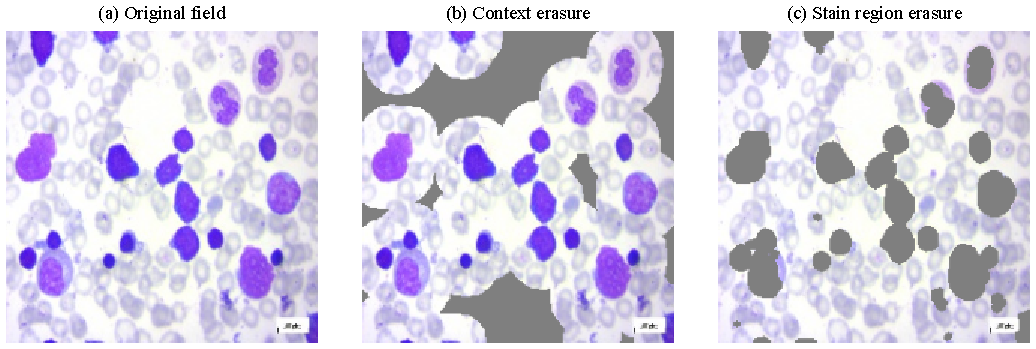
\includegraphics[width=.98\textwidth]{interventions.pdf}
\caption{Training interventions from one source image. The stained region remains visible in (b) and is hidden in (c). The two erasures affect the same number of pixels. These automatic regions provide a training hypothesis, not labelled malignant cells or validated nuclear boundaries.}
\label{fig:interventions}
\end{figure*}

\subsection{Area matched evidence regularization}
The ImageNet pretrained YOLOv8 nano classifier supplies a frozen feature vector of 1,280 dimensions $\phi(x)$. Standardization uses original training features only. A linear head produces four logits $z(x)=W\phi(x)+b$. Freezing the representation isolates the proposed training loss from changes in backbone capacity and permits central processing unit (CPU) reproduction.

For true category $y$, define its margin against the remaining categories:
\begin{equation}
m_y(x)=z_y(x)-\log\sum_{k\ne y}\exp z_k(x).
\end{equation}
Area matched evidence regularization (AMER) uses the penalty
\begin{equation}
r_y(x)=
\log\left(1+\exp\left[1-m_y(x_C)+m_y(x_M)\right]\right).
\end{equation}
Minimizing it favours greater support for the true category when stained regions remain visible than when they are erased. The unit margin fixes the scale of this preference; its strength is selected through the coefficient $\lambda$. The complete objective is
\begin{equation}
\mathcal{L}=\tfrac12\langle\ell_y(x)+\ell_y(x_C)\rangle_w
+\lambda\langle r_y(x)\rangle_{w,V}+\tfrac{\alpha}{2}\|W\|_F^2,
\end{equation}
where $\ell_y$ is cross entropy and $\langle\cdot\rangle_w$ denotes a weighted mean with equal total weight per class. The ranking mean uses only the set $V$ of nonempty proposals and is zero if $V$ is empty. Original images and images with context erased share the source label. Images with stain regions erased receive no new benign label, since erasure does not establish absence of disease. The loss specifies an evidence preference rather than a causal disease model.

\subsection{Controls, fitting and inference}
Five families use the same representation, source split and fitting routine: classification of original images; matched context augmentation without ranking; full context augmentation without ranking; AMER; and AMER with the entire complement erased instead of equal area context. The last family tests area matching while retaining the ranking objective. All controls are fitted afresh; the earlier experimental head is not substituted for the new control trained on original images.

For each family, $\alpha$ ranges over $0.0001$, $0.001$ and $0.01$. Ranking families additionally use $\lambda\in\{0.1,1.0\}$. These small logarithmic grids compare regularization strengths within a fixed fitting budget. We fit the heads deterministically from zero using the limited memory Broyden, Fletcher, Goldfarb and Shanno optimizer with all training samples and a budget of 2,000 iterations. Selection uses validation macro F1, then negative log likelihood, then stronger regularization; nonconverged candidates are ineligible. Macro F1 averages the harmonic mean of precision and recall equally over the categories. One temperature fitted on validation data calibrates the selected logits \cite{guo}. Scikit-learn supplies metric implementations \cite{sklearn}.

All family choices and artifact hashes are saved before new test prediction. Inference requires only $\phi(x)$ and the selected head, with no intervention images or second backbone pass. Binary ALL support sums the three malignant probabilities. The application can request review using a confidence threshold selected on validation data, but this reporting option is not the proposed methodological contribution.

\subsection{Measurements and fixed perturbations}
Detection average precision (AP) summarizes precision over recall; mean AP (mAP) averages over classes. We evaluate intersection over union (IoU) 0.50 and the range 0.50 to 0.95 \cite{voc,coco}. IoU is shared box area divided by combined box area. ALL evaluation reports accuracy across four categories, macro F1, Matthews correlation coefficient (MCC), binary sensitivity and specificity \cite{gorodkin,chicco}. Sensitivity measures correctly flagged ALL images; specificity measures correctly labelled benign images.

The fixed conditions are original images, Gaussian blur with a $5\times5$ kernel and standard deviation one, and global blue, green and red gains of $(0.90,1,1.10)$. A fourth condition applies gains $(0.75,1,1.25)$ only outside the original stain proposal, preserving proposed evidence pixels exactly. Intensities are clipped to the valid range. The blur probes loss of detail; the colour gains probe global and sensitivity to context. These engineering stress settings do not represent calibrated laboratory variation. No parameter is retuned on them. Paired differences use 2,000 bootstrap resamples of source groups, retaining all members of each sampled group. These intervals quantify uncertainty across image groups and do not resolve patient dependence or test reuse.

\begin{figure*}[t]
\centering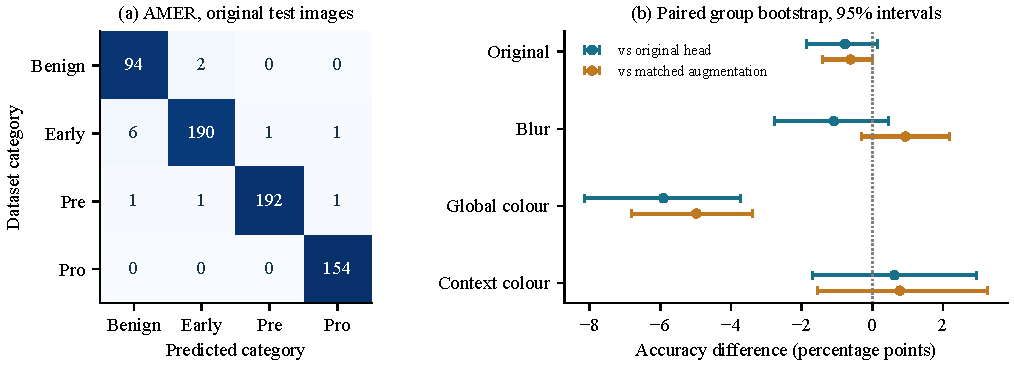
\includegraphics[width=.98\textwidth]{findings.pdf}
\caption{Recorded results, with all 643 test images retained. The confusion matrix shows absolute counts. Difference intervals compare the proposed model with the original image and ordinary augmentation controls; the zero line makes uncertain or negative differences visible. These are exploratory comparisons of image groups.}
\label{fig:findings}
\end{figure*}

\section{Results}
\subsection{Cell analysis}
The detector achieves mAP 0.910 at IoU 0.50 and 0.621 across the stricter range on 72 BCCD test fields. Values for each category are shown in Table~\ref{tab:detector}. The primary normal WBC crop model correctly classifies 55 of 63 sources, or 87.3\%, with a 95\% Wilson interval of 76.9\% to 93.4\% \cite{wilson}. The complete detector and subtype cascade correctly labels 54 true WBCs, with three unmatched predictions. These results concern the cell source dataset and do not measure combined clinical accuracy on ALL fields.

\begin{table}[!t]
\caption{Cell Detection on 72 Test Fields}
\label{tab:detector}\centering\footnotesize
\begin{tabular}{@{}lrrr@{}}
\toprule Category & Objects & AP at 0.50 & AP at 0.50 to 0.95\\\midrule
RBC & 805 & 0.864 & 0.616\\
WBC & 71 & 0.962 & 0.770\\
Platelet & 69 & 0.903 & 0.476\\\midrule
All classes & 945 & 0.910 & 0.621\\\bottomrule
\end{tabular}\end{table}

\subsection{ALL training comparisons}
All 21 fitting candidates converged under the final optimization budget. Validation selected $\alpha=0.0001$ and $\lambda=0.1$ for AMER. Table~\ref{tab:accuracy} reports every family under every fixed condition. On original images, AMER achieves \AmerClean\% accuracy and macro F1 \AmerFone, compared with \OriginalClean\% for the head trained on original images and \AugClean\% for matched augmentation. Its binary counts are \AmerTP\ true positives, \AmerFN\ false negatives, \AmerTN\ true negatives and \AmerFP\ false positives. Sensitivity is \AmerSensitivity\% and specificity is \AmerSpecificity\% (Table~\ref{tab:clean}). All results include every test image, before any review rejection.

\begin{table}[!t]
\caption{Accuracy Across Four Categories Under Fixed Conditions (\%)}
\label{tab:accuracy}\centering\footnotesize
\setlength{\tabcolsep}{3pt}
\begin{tabular}{@{}lrrrr@{}}
\toprule Training & Original & Blur & Global & Context\\\midrule
\AccuracyRows
\bottomrule
\end{tabular}
\par\smallskip\scriptsize Global and Context denote global colour and changes to context colour, respectively.
\end{table}

\begin{table}[!b]
\caption{ALL Metrics on Original Test Images}
\label{tab:clean}\centering\footnotesize
\setlength{\tabcolsep}{2pt}
\begin{tabular}{@{}lrrrr@{}}
\toprule Training & F1 & MCC & Sens. (\%) & Spec. (\%)\\\midrule
\CleanRows
\bottomrule
\end{tabular}
\par\smallskip\scriptsize F1 is the macro average; sensitivity and specificity concern the binary ALL decision.
\end{table}

\subsection{Effects of ranking and area matching}
AMER changes accuracy on original images from 98.8\% to 98.0\%. Its 0.6 percentage point gain under context colour changes has a paired interval crossing zero. Against matched augmentation, the corresponding gain is 0.8 points and is also uncertain. Under global colour changes, AMER loses 5.9 points relative to training on original images, with the entire interval below zero (Table~\ref{tab:difference} and Fig.~\ref{fig:findings}). Thus the observed context gain does not establish greater robustness overall.

Full context augmentation reaches 93.3\% under blur and 78.2\% under context colour changes, whereas AMER reaches 89.7\% and 74.2\%. Adding ranking to full context augmentation lowers these values to 93.2\% and 75.0\%. Area matching also has no consistent advantage across the conditions. These controls show why an apparent improvement under one transformation is insufficient to validate the evidence assumption. No model family is selected retrospectively from the test outcomes.


\begin{table}[!t]
\caption{AMER Accuracy Differences and 95\% Group Intervals}
\label{tab:difference}\centering\footnotesize
\setlength{\tabcolsep}{3pt}
\begin{tabular}{@{}lrr@{}}
\toprule Condition & vs original & vs matched aug.\\\midrule
\DifferenceRows
\bottomrule
\end{tabular}
\par\smallskip\scriptsize Values are percentage points. Intervals crossing zero do not establish a difference under this resampling analysis.
\end{table}



\section{Discussion and Limitations}
The central finding is that matching erased area does not, by itself, make automatic stain proposals an effective training target in this experiment. The supervised margin formulation makes this assumption measurable against ordinary augmentation. It extends evidence training to the available ALL image labels, while building on established explanation constraints, object and context interventions, and comparison of matched regionss \cite{ross,chang,evidencerl}.

Equal area controls the number of altered pixels, but not mask geometry or visual impact. Saturation proposals can include RBCs or exclude weakly stained structures. They are neither annotations of malignant cells nor validated nuclei, and erased images may depart from the natural image distribution. The lower accuracy under global colour changes is consistent with an imperfect evidence target, although the experiment cannot identify its biological cause. Stronger region annotations would allow this explanation to be tested.

The source audit reduces observable duplication but cannot recover missing patient identifiers or eliminate shared acquisition cues. The test partition was previously examined, so the extension needs independent confirmation. The cell detector is inherited, with a known historical validation overlap; the normal WBC test set includes only three monocytes and four lymphocytes. The available datasets do not jointly label cell boxes and ALL categories, so combined accuracy is not established. Larger annotated cell resources, including Raabin WBC, can support better region models, but are not substitutes for an external ALL evaluation \cite{raabin,acevedo,claim}.

\section{Conclusion}
We presented a blood cell analysis system and an evidence regularizer for ALL based on equal area stain and context erasures. Its supervised margin loss requires no expert region labels or additional inference pass. The controlled comparison establishes a clear limit: the proposed ranking term did not outperform training on original images overall, despite 98.0\% clean accuracy. This result supports testing evidence constraints against augmentation controls rather than assuming that region guidance improves screening. External data from separate patients and validated region annotations are the next requirements for assessing generalization.

\section*{Acknowledgment}
The authors thank Rangana W. G. for supervising this project.

\IEEEtriggeratref{11}
\begin{thebibliography}{99}
\bibitem{acevedo} A. Acevedo, A. Merino, S. Alférez, Á. Molina, L. Boldú, and J. Rodellar, ``A dataset of microscopic peripheral blood cell images for development of automatic recognition systems,'' \emph{Data Brief}, vol. 30, Art. no. 105474, 2020, doi: \nolinkurl{10.1016/j.dib.2020.105474}.

\bibitem{matek} C. Matek, S. Schwarz, K. Spiekermann, and C. Marr, ``Human-level recognition of blast cells in acute myeloid leukaemia with convolutional neural networks,'' \emph{Nat. Mach. Intell.}, vol. 1, no. 11, pp. 538-544, 2019, doi: \nolinkurl{10.1038/s42256-019-0101-9}.

\bibitem{ghader} M. Ghaderzadeh, M. Aria, A. Hosseini, F. Asadi, D. Bashash, and H. Abolghasemi, ``A fast and efficient CNN model for B-ALL diagnosis and its subtypes classification using peripheral blood smear images,'' \emph{Int. J. Intell. Syst.}, vol. 37, no. 8, pp. 5113-5133, 2022, doi: \nolinkurl{10.1002/int.22753}.

\bibitem{bccd} Shenggan, ``BCCD Dataset,'' GitHub repository, 2018. [Online]. Available: \url{https://github.com/Shenggan/BCCD_Dataset}

\bibitem{mooney} P. T. Mooney, ``Blood Cell Images,'' Kaggle dataset, 2018. [Online]. Available: \url{https://www.kaggle.com/datasets/paultimothymooney/blood-cells}

\bibitem{all_data} M. Aria, ``Acute Lymphoblastic Leukemia (ALL) image dataset,'' Kaggle dataset, 2021. [Online]. Available: \url{https://www.kaggle.com/datasets/mehradaria/leukemia}

\bibitem{kapoor} S. Kapoor and A. Narayanan, ``Leakage and the reproducibility crisis in machine-learning-based science,'' \emph{Patterns}, vol. 4, no. 9, Art. no. 100804, 2023, doi: \nolinkurl{10.1016/j.patter.2023.100804}.

\bibitem{leakage_questions} J. Bernett \emph{et al.}, ``Guiding questions to avoid data leakage in biological machine learning applications,'' \emph{Nat. Methods}, vol. 21, no. 8, pp. 1444-1453, 2024, doi: \nolinkurl{10.1038/s41592-024-02362-y}.

\bibitem{geirhos} R. Geirhos \emph{et al.}, ``Shortcut learning in deep neural networks,'' \emph{Nat. Mach. Intell.}, vol. 2, no. 11, pp. 665-673, 2020, doi: \nolinkurl{10.1038/s42256-020-00257-z}.

\bibitem{viewstudy} R. Abdallat, O. Al-Bataineh, A. M. Alqudah, and A. Alfraihat, ``An Artificial Intelligence Framework for Detection of Leukemia with Comparison Between Segmented and Non-Segmented Images,'' \emph{Sensors}, vol. 26, no. 19, Art. no. 6290, 2026, doi: \nolinkurl{10.3390/s26196290}.

\bibitem{biomarker} A. Askari Farsangi, A. Sharifi-Zarchi, and M. H. Rohban, ``Novel Pipeline for Diagnosing Acute Lymphoblastic Leukemia Sensitive to Related Biomarkers,'' \emph{arXiv:2307.04014}, revised 2025. \url{https://arxiv.org/abs/2307.04014}

\bibitem{resnet} K. He, X. Zhang, S. Ren, and J. Sun, ``Deep Residual Learning for Image Recognition,'' in \emph{Proc. IEEE CVPR}, pp. 770-778, 2016, doi: \nolinkurl{10.1109/cvpr.2016.90}.

\bibitem{yolo} J. Redmon, S. Divvala, R. Girshick, and A. Farhadi, ``You Only Look Once: Unified, Real-Time Object Detection,'' in \emph{Proc. IEEE CVPR}, pp. 779-788, 2016, doi: \nolinkurl{10.1109/cvpr.2016.91}.

\bibitem{ultralytics} Ultralytics, ``YOLOv8,'' Model documentation. [Online]. Available: \url{https://docs.ultralytics.com/models/yolov8/} (accessed Oct. 11, 2026).

\bibitem{ross} A. S. Ross, M. C. Hughes, and F. Doshi-Velez, ``Right for the Right Reasons: Training Differentiable Models by Constraining Their Explanations,'' in \emph{Proc. IJCAI}, pp. 2662-2670, 2017, doi: \nolinkurl{10.24963/ijcai.2017/371}.

\bibitem{chang} C. H. Chang, G. A. Adam, and A. Goldenberg, ``Towards Robust Classification Model by Counterfactual and Invariant Data Generation,'' in \emph{Proc. IEEE CVPR}, 2021, doi: \nolinkurl{10.1109/CVPR46437.2021.01496}.

\bibitem{evidencerl} H. Huang \emph{et al.}, ``Evidence-RL: Towards Evidence-intensive Visual Reasoning,'' \emph{arXiv:2608.08021}, 2026. \url{https://arxiv.org/abs/2608.08021}

\bibitem{keras} Keras Team, ``NumpyArrayIterator: image augmentation filename construction,'' Keras Preprocessing source code. [Online]. Available: \url{https://github.com/keras-team/keras-preprocessing/blob/master/keras_preprocessing/image/numpy_array_iterator.py} (accessed Oct. 11, 2026).

\bibitem{lowe} D. G. Lowe, ``Distinctive image features from scale-invariant keypoints,'' \emph{Int. J. Comput. Vis.}, vol. 60, no. 2, pp. 91-110, 2004, doi: 10.1023/B:VISI.0000029664.99615.94.

\bibitem{claim} A. S. Tejani \emph{et al.}, ``Checklist for Artificial Intelligence in Medical Imaging (CLAIM): 2024 Update,'' \emph{Radiol. Artif. Intell.}, vol. 6, no. 4, Art. no. e240300, 2024, doi: \nolinkurl{10.1148/ryai.240300}.

\bibitem{imagenet} O. Russakovsky \emph{et al.}, ``ImageNet Large Scale Visual Recognition Challenge,'' \emph{Int. J. Comput. Vis.}, vol. 115, no. 3, pp. 211-252, 2015, doi: \nolinkurl{10.1007/s11263-015-0816-y}.

\bibitem{adamw} I. Loshchilov and F. Hutter, ``Decoupled weight decay regularization,'' in \emph{Proc. ICLR}, 2019. \url{https://arxiv.org/abs/1711.05101}

\bibitem{otsu} N. Otsu, ``A Threshold Selection Method from Gray-Level Histograms,'' \emph{IEEE Trans. Syst., Man, Cybern.}, vol. 9, no. 1, pp. 62-66, 1979, doi: \nolinkurl{10.1109/tsmc.1979.4310076}.

\bibitem{guo} C. Guo, G. Pleiss, Y. Sun, and K. Q. Weinberger, ``On calibration of modern neural networks,'' in \emph{Proc. ICML}, vol. 70, 2017, pp. 1321-1330.

\bibitem{sklearn} F. Pedregosa \emph{et al.}, ``Scikit-learn: Machine learning in Python,'' \emph{J. Mach. Learn. Res.}, vol. 12, pp. 2825-2830, 2011.

\bibitem{voc} M. Everingham, L. Van Gool, C. K. I. Williams, J. Winn, and A. Zisserman, ``The Pascal Visual Object Classes (VOC) Challenge,'' \emph{Int. J. Comput. Vis.}, vol. 88, no. 2, pp. 303-338, 2010, doi: \nolinkurl{10.1007/s11263-009-0275-4}.

\bibitem{coco} T. Y. Lin \emph{et al.}, ``Microsoft COCO: Common Objects in Context,'' in \emph{Proc. ECCV}, pp. 740-755, 2014, doi: \nolinkurl{10.1007/978-3-319-10602-1_48}.

\bibitem{gorodkin} J. Gorodkin, ``Comparing two K-category assignments by a K-category correlation coefficient,'' \emph{Comput. Biol. Chem.}, vol. 28, no. 5-6, pp. 367-374, 2004, doi: \nolinkurl{10.1016/j.compbiolchem.2004.09.006}.

\bibitem{chicco} D. Chicco and G. Jurman, ``The advantages of the Matthews correlation coefficient (MCC) over F1 score and accuracy in binary classification evaluation,'' \emph{BMC Genomics}, vol. 21, no. 1, Art. no. 6, 2020, doi: \nolinkurl{10.1186/s12864-019-6413-7}.

\bibitem{wilson} E. B. Wilson, ``Probable Inference, the Law of Succession, and Statistical Inference,'' \emph{J. Amer. Stat. Assoc.}, vol. 22, no. 158, pp. 209-212, 1927, doi: \nolinkurl{10.1080/01621459.1927.10502953}.

\bibitem{raabin} Z. M. Kouzehkanan \emph{et al.}, ``A large dataset of white blood cells containing cell locations and types, along with segmented nuclei and cytoplasm,'' \emph{Sci. Rep.}, vol. 12, no. 1, Art. no. 1123, 2022, doi: \nolinkurl{10.1038/s41598-021-04426-x}.
\end{thebibliography}

\end{document}
